%%%%%%%%%%%%%%%%%%%%%%%%%%%%%%%%%%%%%%%%%
% University Assignment Title Page 
% LaTeX Template
% Version 1.0 (27/12/12)
%
% This template has been downloaded from:
% http://www.LaTeXTemplates.com
%
% Original author:
% WikiBooks (http://en.wikibooks.org/wiki/LaTeX/Title_Creation)
%
% License: CC BY-NC-SA 3.0 (http://creativecommons.org/licenses/by-nc-sa/3.0/)
% 
% Instructions for using this template:
% This title page is capable of being compiled as is. This is not useful for 
% including it in another document. To do this, you have two options: 
%
% 1) Copy/paste everything between \begin{document} and \end{document} 
% starting at \begin{titlepage} and paste this into another LaTeX file where you 
% want your title page.
% OR
% 2) Remove everything outside the \begin{titlepage} and \end{titlepage} and 
% move this file to the same directory as the LaTeX file you wish to add it to. 
% Then add \input{./title_page_1.tex} to your LaTeX file where you want your
% title page.
%
%%%%%%%%%%%%%%%%%%%%%%%%%%%%%%%%%%%%%%%%%
%\title{Title page with logo}
%----------------------------------------------------------------------------------------
%	PACKAGES AND OTHER DOCUMENT CONFIGURATIONS
%----------------------------------------------------------------------------------------
\documentclass[14pt]{extarticle}
%Paquetes para idioma español y codifcación UTF8
\usepackage[spanish]{babel}
\usepackage[utf8]{inputenc}
\usepackage{csquotes}

%%% BIBLATEX
\usepackage{biblatex}
%%% BIBLIOGRAPHY
\addbibresource{references.bib}

%fuente 'fourier'
\usepackage{fourier}
%paquete para URLs
\usepackage{url}
\usepackage[hidelinks]{hyperref}
%paquete para ubicar las imágenes
\usepackage{float}
%paquete para imágenes y en dónde las tiene que buscar
\usepackage{graphicx}
\graphicspath{{images/}}
%paquete para epígrafes
\usepackage{subcaption}
%paquete para definir los márgenes de la hoja
\usepackage[left=1.5cm,right=1.5cm,top=3cm,bottom=3cm]{geometry}
%paquete para poner todos y comentarios
\usepackage[colorinlistoftodos]{todonotes}
%paquete para trabajar con código
\usepackage{listings}
%paquete para trabajar con colores y definir propios
\usepackage{color}

%paquete para el checkmark y la cruz
\usepackage{pifont}
%paquete para el signo de copyright
\usepackage{textcomp}

%Cabeceras
\usepackage{fancyhdr}
\pagestyle{fancy}
\fancyhead[L]{Sistemas distribuidos, 2018}
\fancyhead[C]{}
\fancyhead[R]{UNPSJB}

\fancyfoot[R]{SERRUYA ALOISI, TOLEDO MARGALEF}
\fancyfoot[L]{Trabajo de laboratorio}

%Comando para poner doble comillas más fácil
\newcommand{\dq}[1]{``#1''}
\newcommand{\cmark}{\ding{51}}
\newcommand{\xmark}{\ding{55}}

\definecolor{comment-green}{rgb}{0,0.5,0}
\definecolor{bg-light-gray}{HTML}{E9E9E9}
\definecolor{bg}{HTML}{D0B698}

\lstdefinestyle{MyStyle}{
    backgroundcolor=\color{bg},
    basicstyle=\ttfamily,
  	keywordstyle=\bfseries\color{white},
    stringstyle=\color{blue},
    commentstyle=\color{comment-green}\itshape,
    numberstyle=\color{gray},
    identifierstyle=\color{black},
    rulecolor=\color{gray},
    showstringspaces=false,
    escapeinside={\%*}{*)},
    morekeywords={},
    otherkeywords={},
    breaklines=true,
    frame=trbl, 
    framexleftmargin=25pt,
    numbers=left,
    xleftmargin=\parindent,
    frameround=tttt,
    captionpos=b,
    % re tirado de los pelos, pero es lo que hay
    % sacado de:
    % https://tex.stackexchange.com/questions/24528/having-problems-with-listings-and-utf-8-can-it-be-fixed
    inputencoding=utf8,
    extendedchars=true,
    literate={á}{{\'a}}1 {é}{{\'e}}1 {í}{{\'{\i}}}1 {ó}{{\'o}}1 {ú}{{\'u}}1 {Á}{{\'A}}1 {É}{{\'E}}1 {Í}{{\'I}}1 {Ó}{{\'O}}1 {Ú}{{\'U}}1 {ü}{{\"u}}1 {Ü}{{\"U}}1 {ñ}{{\~n}}1 {Ñ}{{\~N}}1 {¿}{{?``}}1 {¡}{{!``}}1
}


\begin{document}

%%%%%%%%%%%%%%%%%%%%%%%%%%%%%%%%%%%%%%%%%%%%
% En 'titlepage.tex' se encuentra la página de título
%%%%%%%%%%%%%%%%%%%%%%%%%%%%%%%%%%%%%%%%%%%%
\begin{titlepage}

    \newcommand{\HRule}{\rule{\linewidth}{0.5mm}} % Defines a new command for the horizontal lines, change thickness here

    \center % Center everything on the page
     
    %----------------------------------------------------------------------------------------
    %	HEADING SECTIONS
    %----------------------------------------------------------------------------------------

    \textsc{\LARGE UNPSJB}\\[1cm] % Name of your university/college
    \textsc{\Large Licenciatura en Sistemas OPGCPI}\\[0.5cm] % Major heading such as course name
    \textsc{\large Sistemas distribuidos}\\[0.5cm] % Minor heading such as course title

    %----------------------------------------------------------------------------------------
    %	TITLE SECTION
    %----------------------------------------------------------------------------------------

    \HRule \\[0.4cm]
    {\huge \bfseries Trabajo de Laboratorio}\\[0.4cm] % Title of your document
    {\large \bfseries Coso}\\[0.4cm] % Title of your document
    \HRule \\[1.5cm]
     
    %----------------------------------------------------------------------------------------
    %	AUTHOR SECTION
    %----------------------------------------------------------------------------------------


    \begin{minipage}[l]{0.5\textwidth}
        \begin{flushleft}
            \textbf{\textsf{Cátedra}}\\
            \large Mg. Ing. Ricardo López\\ 
            \large Lic. Cristian Parise\\ 
            \linespread{4}
            \end{flushleft}
    \end{minipage}
    \begin{minipage}[l]{0.4\textwidth}
        \begin{flushright}
            \textbf{\textsf{Integrantes:}}\\
            \linespread{1}
            \large Luciano Serruya Aloisi\\
            \large Pablo Toledo Margalef\\
        \end{flushright}
    \end{minipage}\\[1.5cm]

    % If you don't want a supervisor, uncomment the two lines below and remove the section above
    %\Large \emph{Author:}\\
    %John \textsc{Smith}\\[3cm] % Your name

    %----------------------------------------------------------------------------------------
    %	DATE SECTION
    %----------------------------------------------------------------------------------------

    {\large \today}\\[1cm] % Date, change the \today to a set date if you want to be precise

    %----------------------------------------------------------------------------------------
    %	LOGO SECTION
    %----------------------------------------------------------------------------------------

    
\includegraphics[scale=1]{logoUnpsjb.png}\\[0.5cm] % Include a department/university logo - this will require the graphicx package
     
    %----------------------------------------------------------------------------------------

    % \vfill % Fill the rest of the page with whitespace

\end{titlepage}


%%%%%%%%%%%%%%%%%%%%%%%%%%%%%%%%%%%%%%%%%%%%
% INDICE
%%%%%%%%%%%%%%%%%%%%%%%%%%%%%%%%%%%%%%%%%%%%
\clearpage
\tableofcontents
\clearpage 

\lstset{style=javastyle}

\section{Ejercicio 1 - Calculadora implementada con RMI}

\emph{El código fuente y las capturas de paquetes se pueden encontrar en los directorios \dq{ej1/src} y \dq{ej1/pcaps}, respectivamente} 

~\\

El servidor de la presente aplicación publica dos servicios distintos, con el fin de emular una calculadora: \emph{SumaResta}, y \emph{MultiplicacionDivision}; el primero implementa la interfase \texttt{ISumaResta} y el segundo \texttt{IMultiplicacionDivision} (ambas interfases extienden la interfase \texttt{Remote}). 

El cliente (clase \texttt{Cliente}) consiste en un intermediario entre la aplicación de consola (clase \texttt{CLICliente}) y el servidor; el \emph{parser} de línea de comandos toma los argumentos y según el operador ingresado llama a alguno de los métods del \emph{Cliente} (\texttt{sumar}, \texttt{restar}, \texttt{multiplicar}, \texttt{dividir}). Estas operaciones son realizadas por el \textbf{servidor}, y no por el \textbf{cliente}.

A partir de las capturas realizadas con el analizador de protocolos \emph{Wireshark}, se puede deducir lo siguiente:

\begin{itemize}
    \item Las interacciones tanto del servidor (para publicar servicios) como del cliente (para consumir esos servicios) se hace a través del \textbf{RMIregistry} 
    \item RMIregistry escucha en un puerto bien conocido para ambas partes - escucha peticiones en el puerto \textbf{1099}
    \item Para recuperar el objeto remoto, el cliente primero se comunica con el RMIregistry (éste último le indica en qué puerto está escuchando el objeto remoto)
    \item El cliente recupera un \emph{objeto remoto} invocando el método \texttt{lookup} de la clase \texttt{Naming} indicándole el \emph{URI} del objeto - envía una petición al puerto de escucha que le indicó RMIregistry
    \item El \emph{URI} se compone de la dirección donde se encuentra el servidor, el puerto de escucha de RMIregistry, y el nombre del servicio publicado por el servidor
    \item Toda la comunicación de RMIregistry es a través de \textbf{TCP} 
\end{itemize}

\subsection{Numeración de paquetes de la captura \emph{pcapng}}

\emph{El archivo de la captura es \dq{rmi-sumaresta.pcapng} - abrir con Wireshark o con \texttt{tcpdump}} 

A continuación se enumeran los distintos paquetes que fluyen por la red entre el servidor y el RMIregistry en el momento en el que el primero publica los servicios. También se indican los paquetes cuándo un cliente recupera el objeto remoto, y por último los paquetes que representan el llamado a un método remoto: 

\begin{itemize}
    \item 1-29: servidor publica servicios. Para ello se comunica directamente con el RMIregistry (puerto 1099)
    \item 32-60: cliente recupera el objeto remoto que implementa la interfase \texttt{ISumaResta}. Primero se comunica con RMIregistry en el puerto 1099, y luego se comunica con el objeto remoto en el puerto 39529 
    \item 70-87: invocación de método remoto. Se comunica directamente con el objeto remoto al puerto 39529.
\end{itemize}

\section{Ejercicio 2 - RFS implementado con RMI}

Utilizando RMI, se puede implementar un \emph{sistema de archivos remotos} fácilmente. Para ello, se tomó como proyecto base la implementación realizada en el trabajo de laboratorio anterior y se lo modificó acordemente para que utilice RMI.

En esta nueva versión, la estructura del proyecto se vio fuertemente alterada; en la versión implementada con \emph{sockets}, toda la infraestructura de comunicación entre cliente y servidor fue desarrollada desde cero, enviando objetos \texttt{RFSArgument} y reaccionando según el tipo de argumento del que se trate. De esta forma se lograba transmitir alrededor de 400 MB de un archivo en 37 minutos, aproximadamente.

Utilizando RMI, el desarrollo tanto del cliente como del servidor no tiene que preocuparse por la comunicación entre estos, ya que RMI se encarga de ello. La primer modificación que se puede ver es que \textbf{las clases de \emph{stub} desaparecieron} (ya no son necesarias para esta versión). Cuando se instancia la clase \texttt{Client} (encargada de hacer las llamadas al \texttt{fileSystem}), solicita el objeto remoto publicado por el servidor a través de la clase \texttt{Naming}.

Ejecutando la misma prueba que en las versiones de RPC y la de \emph{sockets} (transferir un archivo de texto de 3.9 GB, utilizando un buffer de transferencia de 8 KB), la implementación con RMI es considerablemente superior - la transferencia del archivo demoró \textbf{solamente 33 segudos}, frente a 17 minutos de la versión de RPC y aproximadamente 37 minutos para transferir 400 MB con la versión de \emph{sockets}.

\begin{figure}[H]
    \centering
    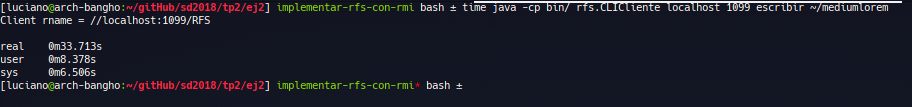
\includegraphics[width=\linewidth]{archivo-transferido-rmi.png}
    \caption{Transferencia del archivo de texto con la versión de RMI}
\end{figure}

Por otro lado, los servicios publicados con RMI no permiten trabajar con funciones que utilicen argumentos de salida o entrada/salida. Por lo tanto, la interfase \texttt{IFileSystem} tuvo que ser modificada (la operación \texttt{read}, en particular) para eliminar los argumentos de salida. En esta versión, la operación \texttt{read} recibe un archivo del cual leer y una cantidad de bytes, y devuelve un \emph{arreglo de bytes} con los datos leídos.   


\section{Ejercicio 3 - Servidores concurrentes - Comparación RPC y RMI}

El principal problema con el que tienen que lidiar los servidores concurrentes es el del \textbf{acceso a los recursos}. Este problema consiste en administrar los recursos disponbiles para que los clientes los puedan solicitar y que mantengan un estado consistente. 

Para trabajar con una situación de este tipo en un sistema distribuido implementado con Java y RMI, el lenguaje provee de la palabra reservada \texttt{synchronized}. Cuando un hilo está ejectuando un método definido como \emph{sincronizado}, todos los otros hilos que quieran ejectuar ese método \textbf{del mismo objeto} serán bloqueados (se suspende su ejecución) hasta que finalice la ejecución del primer hilo \autocite{SynchronizedMethods}

RPC y RMI son comparable en cuanto a que ambos implementan una capa de \emph{middleware} que resulta transparente para el programador. Utilizando estas herramientas, se logra desarrollar un sistema distribuido trabajando con objetos (RMI) o llamadas a funciones y registros (RPC) de forma que parecen ser locales, pero realmente se están ejectuando de forma remota. Todo el \dq{andamiaje} necesario para comunicar un cliente con un servdior (como el implementado en el trabajo de laboratorio anterior) ya es implementado por la herramienta.

Sin embargo, no se podría decir que trabajan en \emph{exactamente el mismo nivel de abstracción}, pero la diferencia no se debe a la herramienta, sino al \textbf{lenguaje para el cual están implementados} (C en el caso de RPC, y Java para RMI).  

Algunas diferencias entre RPC y RMI son las siguientes:

\begin{itemize}
    \item RMI no utiliza un lenguaje propio para definir las interfaces de las funciones y las estructuras de datos, sino que se definen como interfases de Java
    \item En RPC no se publican los servicios bajo una \emph{URL}; \texttt{rpcgen} genera el archivo \texttt{.h} con las firmas de las funciones remotas para llamarlas desde algún cliente  
    \item RMI publica objetos (que implementan la funcionalidad del servicio), los cuales serán requeridos por los clientes y las funciones remotas serán invocadas a través de los métodos del objeto remoto.
\end{itemize}


Con respecto al manejo de concurrencia de RMI, se puede verificar que crea \textbf{un hilo por referencia a objeto remoto}. Un experimento posible para demostrar esto consiste en modificar la clase \emph{SumaResta.java} del proyecto del ejercicio anterior de la siguiente manera:

\begin{lstlisting}[title={Modificar el método \texttt{suma} para poder ver el hilo en el que corre}]
    public int suma(int a, int b) {
        long threadId = Thread.currentThread().getId();
        JOptionPane.showMessageDialog(null, 
                String.format("HILO [%d]", threadId));
        return a+b;
    }
\end{lstlisting}

Si se ejecuta varias veces el método \texttt{suma} \textbf{con el mismo cliente}, se podrá ver que siempre se imprime el mismo número de hilo. Se podría ver lo mismo si el mismo cliente ejecuta otro método del objeto remoto (el método \texttt{resta}, por ejemplo).  

\section{Ejercicio 4 - Experimentos con RMI}

\emph{RMI otorga un servicio concurrente en forma automática para el acceso a objetos remotos} 
~\\

Con la modificación realizada al proyecto de la calculadora mostrada en la sección inmediatamente anterior, se puede ver que \textbf{RMI automáticamente otorga un manejo concurrente de los objetos remotos} - cada referencia a un objeto remoto es un hilo distinto en el servidor.

\emph{Las variables de instancia de un determinado objeto remoto, no se “contaminan” con sus equivalentes de otras instancias del mismo objeto a las que se está accediendo en forma concurrente (acceso sincronizado)} 
~\\

Realizando varias modificaciones a la implementación de la calculadora, se pueden realizar varios experimentos para ver que \textbf{se dan condiciones de carrera}. Para poder verlo más claramente, se debe reiniciar el servidor cada vez que se quiera hacer una nueva prueba (\emph{los códigos fuente necesarios para los experimentos se encuentran en el directorio \dq{ej4}}).

Primero se debe ejecutar \texttt{rmiregistry} y el servidor que publica los servicios de suma y resta, y multiplicación y división. Para levantar el servidor, se debe correr el siguiente comando dentro del directorio \dq{ej4}: \texttt{java -cp bin Servidor}. 

Las condiciones de carrera se pueden ver cuando se corren dos clientes a la vez, intercalando las ejecuciones. Primero se debe correr uno, con una operación de suma/resta - se mostrará un mensaje indicando el \dq{estado} del objeto remoto. Dejando ese mensaje abierto, correr el otro cliente con la operación inversa de suma/resta, y ejecutarlo hasta que finalice su ejecución. Luego correr el primero hasta que finalice, y comparar los resultados.

Probando distintas combinaciones de operaciones de suma/resta y operandos se puede ver que se obtienen distintos resultados del \dq{estado} del objeto remoto. A continuación se detalla un experimento concreto para realizar:

\begin{itemize}
    \item Correr \texttt{rmiregistry} y el servidor 
    \item Ejecutar el cliente con el comando \texttt{java -cp bin CLICliente localhost 21 + 9} - No cerrar el primer mensaje. Cuando se ejecuta una suma o una resta, el objeto remoto incrementa un contador
    \item Ejecutar otro cliente con el comando \texttt{java -cp bin CLICliente localhost 30 - 20} - Ejecutar hasta finalizar
    \item Continuar con la ejecución del primer cliente - el resultado final del estado debe ser 2
\end{itemize}

Cabe aclarar que, aunque cada cada cliente tenga \textbf{referencia} al objeto remoto (en este caso, al objeto de la clase \texttt{SumaResta} publicado por el servidor), sigue siendo el mismo objeto, por lo tanto hay un \textbf{único estado}. Para evitar estas condiciones de carrera, se podría modificar los métodos de suma y de resta de tal forma que solamente un cliente los ejecute por vez (que su ejecución sea atómica); de esta forma el estado no terminaría en valores inesperados.  

\emph{Cuando se pasan objetos remotos como parámetros el pasaje es por referencia, contrariamente de cuando se pasan objetos locales (por valor)} 
~\\

Para demostrar este enunciado, se modificó la clase \texttt{Cliente} agregando un método \texttt{wrapperSuma}. Su objetivo es demostrar que el pasaje de los objetos remotos es por referencia, y no por valor.

El resultado de las ejecuciones se debe mantener igual que en las secciones anteriores: por cada operación de suma/resta, se mostrará un contador de cuántas de estas operaciones se han realizado.

\section{Ejercicio 5 - Implementación de Timeout}

Al tener que tratar con servicios remotos el cliente se encuentra atado a la \textbf{disponibilidad} del servidor en cueanto a tiempo para poder atender sus peticiones. Por lo tanto, lo que puede hacer el cliente es fijar un tiempo de espera o \textbf{timeout} para las peticiones que le realice al servidor. De esta forma no se queda esperando indefinidamente a que le respondan.

Para implementar el timeout en el cliente debemos crear una clase \texttt{TimeoutFactory} que cree los sockets de cliente y servidor contemplando un timeout especificado. Y luego hacer que el cliente adopte precauciones con respecto a los tiempos de espera.

\begin{lstlisting}[title={Socket factory que contempla el \textbf{timeout} especificado}]
class TimeoutFactory extends RMISocketFactory {

    private int timeout;

    public TimeoutFactory(int timeout) {
        this.timeout = timeout;
    }

    public Socket createSocket(String host, int port) throws IOException {
        Socket ret = getDefaultSocketFactory().createSocket(host, port);
        ret.setSoTimeout(timeout * 1000);
        return ret;
    }

    public ServerSocket createServerSocket(int port) throws IOException {
        return getDefaultSocketFactory().createServerSocket(port);
    }
}
\end{lstlisting}

Luego, en el cliente, antes de setear el valor del host al cual conectarse para requerir los servicios:

\begin{lstlisting}[title={Utilizar la \texttt{TimeoutFactory} como default para la creación de sockets en el constructor de Cliente}]
    public Cliente(String host) {
        try {
            RMISocketFactory.setSocketFactory(
                new TimeoutFactory(5)
            );
        } catch(IOException e){
            e.printStackTrace();
        }
        this.setHost(host);
    }
\end{lstlisting}

Al utlizar esta nueva implementación se le agregó una pausa de 6 segundos en el servicio de Suma. Luego se ejecutó el cliente requiriendo la suma. Como la espera máxima fijada es de 5 segundos, el servicio falla. Cuando la espera se quita el servicio finaliza exitosamente.

\section{Ejercicio 6 - Relojes}

\emph{Los códigos fuentes necesarios para este ejercicio se encuentran en el directorio \emph{ej6/src}} 

Para implementar el reloj de la hora, primero se definió la interfase \texttt{IReloj} con su único método \texttt{now()}, que devuelve un valor \texttt{long} de Java (pensado para que devuelva la hora en formato EPOCH \footnote{También conocido como \emph{Tiempo UNIX} o \emph{POSIX}, indica el tiempo actual como una aproximación a la cantidad de segundos que pasaron desde las 00 horas (UTC) del 1 de Enero de 1970 \autocite{WikipediaEpoch}}). El servidor publica un servicio como un objeto RMI que devuelve la hora, y la aplicación para lanzar el servidor acepta como parámetro por línea de comandos un corrimiento (tanto positivo como negativo) para aplicar al reloj (\emph{ejecutar la aplicación del servidor con el parámetro \emph{--help} para ver cómo pasar dicho valor}).

El cliente es considerablemente más complejo; no solo tiene una muy sencilla interfaz gráfica, sino que se encarga de pedir al servidor su hora actual, y actualizar su reloj local en base al \textbf{algoritmo de Cristian}. La implementación de este algoritmo se puede hallar en la clase \texttt{ActualizadorDeriva}.

Ahora bien, cuando se ejecuta el cliente, luego de recuperar los parámetros correspondientes de la invocación de línea de comandos, primero inicializa la interfaz gráfica.

Luego, lanza dos hilos nuevos. Uno de ellos (clase \texttt{ActualizadorReloj}) se encargará de actualizar el reloj cada un determinado tiempo (varía según la deriva que tenga el reloj). Este hilo emite el evento necesario para refrescar la interfaz gráfica. El otro hilo (clase \texttt{ActualizadorDeriva}) es el encargado de ir actualizando la deriva del reloj, en base a la diferencia que exista entre el reloj local y el del servidor (sigue el Algoritmo de Cristian).

A continuación se detallan los pasos necesarios para correr la aplicación:

\begin{itemize}
    \item Compilar los códigos fuente valiéndose del archivo \emph{Makefile} disponbile en el directorio \emph{ej6/} - compilar con el comando \texttt{make}.
    \item Correr el \emph{rmiregistry}. Para ello se puede probar alguna de las siguientes opciones:
    \begin{itemize}
        \item Ejecutar el comando \texttt{rmiregistry} estando parado dentro del directorio \emph{bin/} (generado por el comando \texttt{make})  
        \item \texttt{rmiregistry -J--class-path=./bin/} (estando parado en el directorio \emph{ej6})
    \end{itemize}
    \item Correr la aplicación del servidor con \texttt{java -cp bin servidor.MainServidor} (el parámetro \emph{--help} permite ver las distintas banderas con las que cuenta) 
    \item Correr la aplicación del cliente con \texttt{java -cp bin cliente.MainCliente} (al igual que la aplicación del servidor, cuenta con un parámetro de ayuda). 
\end{itemize}

\section{Ejercicio 7 - NTP Servers}

Utilizando un conjunto de clases provistas por la cátedra, \texttt{NtpMessage} para realizar una consulta a un servidor NTP, y \texttt{SntpClient} como base para armar un cliente,  se implementó un nuevo cliente que realiza una serie de consultas a diversos servidores NTP para graficar los offset que se observaban cuando se consulta uno u otro servidor.

Los servidores utilizados fueron:

\begin{center}
    \begin{tabular}{ c }
        \textbf{Server URL} \\
        \hline
        \hline
        pool.ntp.org \\ 
        asia.pool.ntp.org \\
        europe.pool.ntp.org \\
        north-america.pool.ntp.org \\
        oceania.pool.ntp.org \\ 
        south-america.pool.ntp.org \\ 
    \end{tabular}
\end{center}

Se grafica un fragmento a la salida de la serie de pruebas realizadas:

\begin{lstlisting}
|                          - |        - |          - |
|                   Servidor | # prueba |     Offset |
|                          - |        - |          - |
|               pool.ntp.org |        1 | -64.191 ms |
|               pool.ntp.org |        2 | -64.234 ms |
|               pool.ntp.org |        3 | -64.171 ms |
|               pool.ntp.org |        4 | -64.172 ms |
|               pool.ntp.org |        5 | -64.184 ms |
|               pool.ntp.org |        6 | -64.209 ms |
|               pool.ntp.org |        7 | -64.176 ms |
|               pool.ntp.org |        8 | -64.175 ms |
|                          - |        - |          - |
|          asia.pool.ntp.org |        1 | -64.219 ms |
|          asia.pool.ntp.org |        2 | -64.228 ms |
|          asia.pool.ntp.org |        3 | -64.226 ms |
|          asia.pool.ntp.org |        4 | -64.227 ms |
|          asia.pool.ntp.org |        5 | -64.163 ms |
.
.
.
\end{lstlisting}

\section{Ejercicio 8 - Criptografía. Verdadero o Falso}

\begin{itemize}
    \item Verdadero, al ambas partes conocer la clave, en situación de disputa frente a una tercera parte, no puede determinarse quién encriptó el mensaje.
    \item Falso. La encriptación asimétrica, al agregar un overhead sobre la confección del mensaje, disminuye notablemente la eficiencia. Es por eso que se opta por utilizar criptografía asimétrica para la transmisión de una clave que luego se utilizará para llevar adelante una comunicación encriptada simetricamente.
    \item Falso. En ciptografía simétrica sí, pero en asimétrica no. Es más, en PKI las claves públicas pueden estar en público conocimiento. \autocite{WikipediaDigitalSignature}
\end{itemize}

\section{Ejercicio 9 - Firma Digital}

\begin{itemize}
    \item Es necesaria la clave pública del remitente.
    \item Necesito mi clave privada. Utilizando el método de establecimiento de claves que haga falta, como ser Diffie-Hellman. \autocite{WikipediaEmailEncryption}
    \item Requiere la clave pública del remitente para poder encriptar el mail y que pueda desencriptarlo con su clave privada.
\end{itemize}


\section{Ejercicio 10 - PKI}

\begin{itemize}
    \item Mi certificado se encontrará firmado utilizando una clave comprometida que ya no tiene valor de seguridad.
    \item Ahora alguien más puede desencriptar información que era sólo para mí.
    \item Puedo cambiar mi par de llaves. Dicho cambio requiere regenerar mis certificados, para con los demas. Y el hecho de cambiar mi clave pública, procurando que se deje inutilizado el par anterior de claves. En este punto se puede ver una vulnerabilidad, si mediante algún medio se impide el conocimiento del nuevo par de claves, puede haber robo de información \autocite{WikipediaPublicKeyCertificate}
\end{itemize}

\section{Ejercicio 11 - Transacciones distribuidas}

\emph{Explicar cómo el protocolo de compromiso de dos fases para transacciones anidadas, se asegura que si la transacción de nivel superior se compromete, todas las descendientes se comprometen o se abortan} 
~\\

Eeeee

\subsection{Implementación con \emph{JTA}}

\emph{Los códigos fuentes necesarios para este ejercicio se encuentran en el directorio \emph{ej11/src}} 

Esta solución utiliza tanto las librerías estándar de \emph{JDBC} (\emph{Java Database Connectivity}), como de \emph{JTA} (\emph{Java Transaction API}). Debido a la cantidad de código \dq{de andamiaje} necesario para llevar a cabo una operación con \emph{JDBC} y \emph{JTA}, se decidió implementar el paquete \texttt{db} con distintas clases que hagan más sencillo el uso de las librerías (encapsulando su complejidad y presentando una interfaz más simple, enfocada principalmente en el enunciado del ejercicio).   

Para utilizar la aplicación desarrollada, primero se debe contar con las bases de datos necesarias; para esta situación se decidió utilizar \emph{contenedores de Docker} y la herramienta de orquestración de contenedores \emph{docker-compose}. 

Si se desea probar la aplicación, primero se deben crear los contenedores con el comando \texttt{docker-compose up --build -d} (estando parado en el directorio \emph{ej11/}). Con dicho comando se crearán dos contenedores, uno para cada base de datos que se necesita. Cada base de datos ya es inicializada con la tabla \texttt{cuentas} necesaria, y con algunos registros creados.

Por otro lado, para no tener que estar manejando código SQL desde la aplicación de Java, se implementó el paquete \texttt{cuenta}, con las clases \texttt{Cuenta} y \texttt{CuentaObjects}. La primera es una modelación sencilla de la tabla homónima, con sus respectivos campos y tipos de datos, y algunos métodos que implementan una lógica básica (si una cuenta está bloqueada o no, si tiene saldo suficiente para realizar una extracción, depositar o extraer una suma, y actualizar su registro en la base de datos). La segunda se encarga de buscar en la base de datos una cuenta (según un identificador pasado por parámetro), y devolver un objeto \texttt{Cuenta}.

Al igual que en la aplicación del ejercicio 6, se debe compilar el código con el comando \texttt{make}. En este caso, para correr la aplicación no hace falta levantar ningún servidor (solamente los contenedores); entonces una vez compilado el código, se debe ejecutar el siguiente comando:

\begin{lstlisting}[title={Ejemplo de invocación de la aplicación (correr estando parado en el directorio \emph{ej11})}]
java -cp ./bin/:./lib/postgresql-42.2.5.jar app.App 
\end{lstlisting}

La aplicación le pedirá un monto a extraer de una cuenta y depositar en la otra, un identificador de cuenta de la cual extraer (verificará que exista, que la cuenta no esté bloqueada, y que tenga saldo suficiente), y un segundo identificador de una cuenta a la cual depositar (verificando también que no exista ni que esté bloqueada). Luego, realizará la operación y por último, solicitará una confirmación.


%%%%%%%%%%%%%%%%%%%%%%%%%%%%%%%%%%%%%%%%%%%%
% FIN DOCUMENTO, AHORA REFERENCIAS
%%%%%%%%%%%%%%%%%%%%%%%%%%%%%%%%%%%%%%%%%%%%
\clearpage
\printbibliography

\end{document}

